\documentclass[border=10pt]{standalone}

\usepackage{tikz}
\usepackage{tikzsymbols}
\usetikzlibrary{calc,patterns,shapes.geometric}

\def\centerarc[#1](#2)(#3:#4:#5){\draw[#1] ($(#2)+({#5*cos(#3)},{#5*sin(#3)})$) arc (#3:#4:#5);}

\begin{document}
	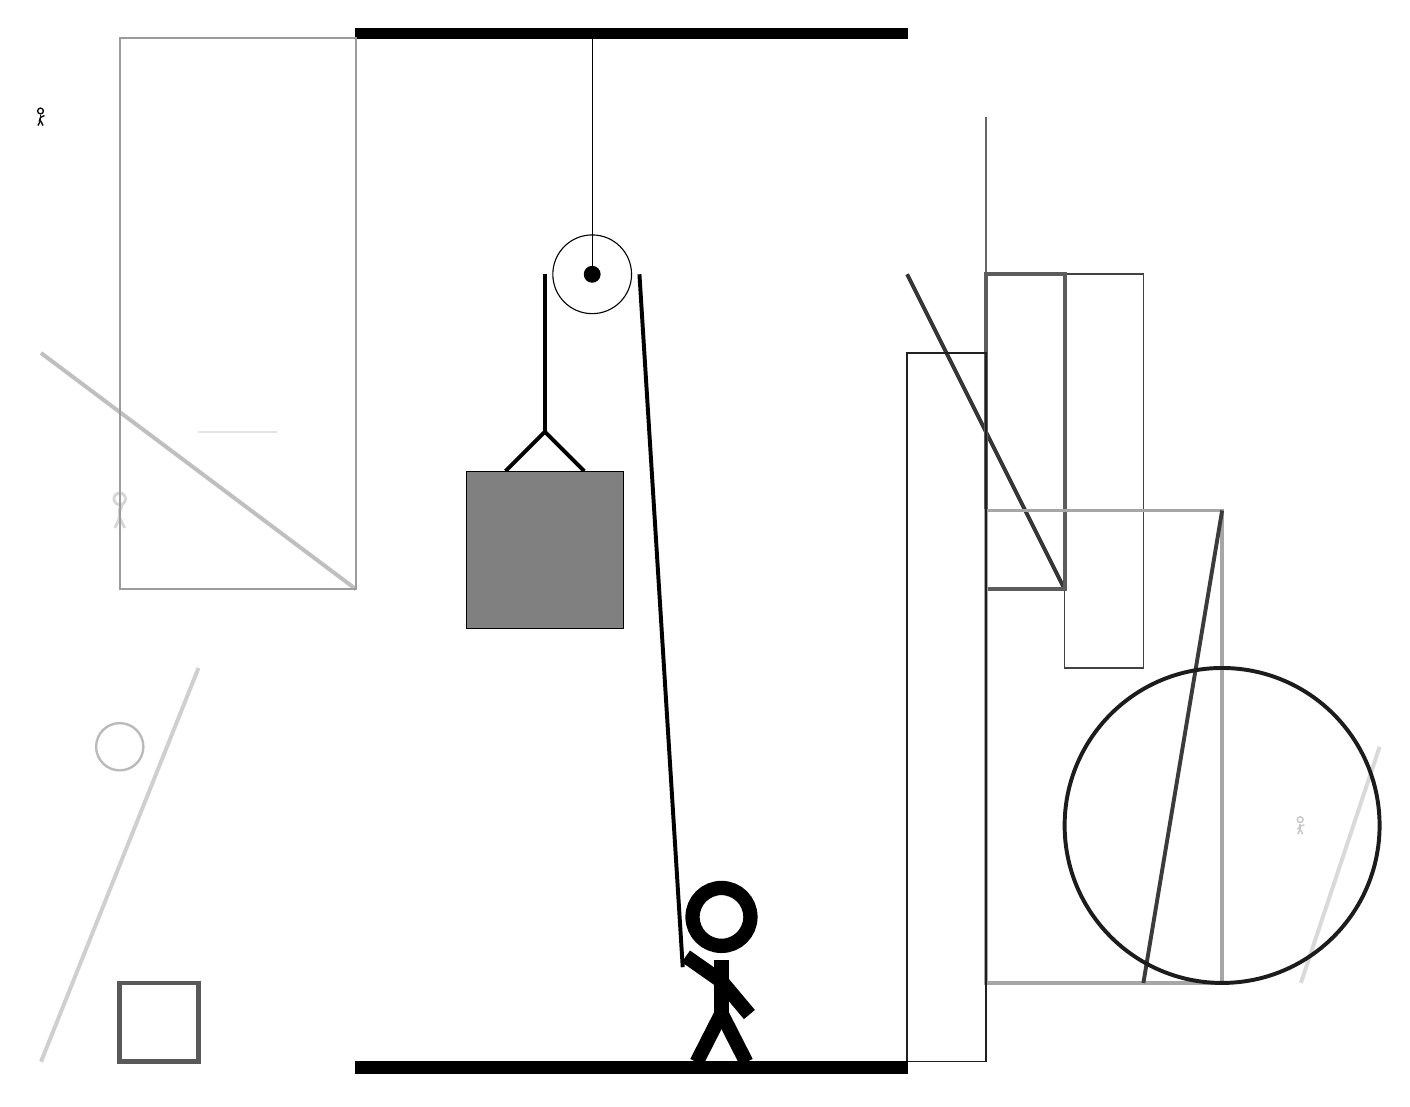
\begin{tikzpicture}
		%%%%% START %%%%%
		
		\draw[fill=black] (-2, 10) rectangle (5, 10.125);
		
		\draw (1, 7) circle (0.5);
		\draw[fill=black] (1, 7) circle (0.1);
		\draw (1, 10) -- (1, 7);
		
		\draw[line width=0.5mm] (-0.1, 4.5) -- (0.4, 5.0) -- (0.9, 4.5);
		\draw[fill=black!50] (-0.6, 4.5) rectangle (1.4, 2.5);
		
		\draw[line width=0.5mm] (0.4, 7) -- (0.4, 5.0);
		\centerarc[line width=0.5mm](1, 7)(0:180:0.6);
		\draw[line width=0.5mm](1.6, 7) -- (2.15, -1.8);
		
		\node at (2.6, -1.9) {\Strichmaxerl[10][-35][-50]};
		
		\draw[line width=0.5mm, color=black!25](-6, 6) -- (-2, 3);
		
		\draw[line width=0.5mm, color=black!19](-4, 2) -- (-6, -3);
		\draw[line width=0.6mm, color=black!65] (-4, -2) rectangle (-5, -3);
		\node[line width=0.3mm, color=black!16] at (-5, 4) {\Strichmaxerl[2][84][72]};
		\draw[line width=0.5mm, color=black!79](7, 3) -- (5, 7);
		\draw[line width=0.3mm, color=black!60] (6, -2) rectangle (6, 9);
		\draw[line width=0.2mm, color=black!74] (7, 7) rectangle (8, 2);
		\draw[line width=0.3mm, color=black!39] (-2, 10) rectangle (-5, 3);
		\draw[line width=0.5mm, color=black!64] (6, 7) rectangle (7, 3);
		\node[line width=0.2mm, color=black!95] at (-6, 9) {\Strichmaxerl[1][72][26]};
		
		\draw[line width=0.5mm, color=black!35] (6, -2) rectangle (9, 4);
		
		\node[line width=0.4mm, color=black!22] at (10, 0) {\Strichmaxerl[1][51][16]};
		\draw[line width=0.2mm, color=black!88] (5, 6) rectangle (6, -3);
		
		\draw [line width=0.3mm, color=black!27](-5, 1) circle (0.3);
		\draw[line width=0.5mm, color=black!15](10, -2) -- (11, 1);
		\draw[line width=0.5mm, color=black!77](8, -2) -- (9, 4);
		
		\draw[line width=0.2mm, color=black!10] (-3, 5) rectangle (-4, 5);
		\draw [line width=0.5mm, color=black!89](9, 0) circle (2.0);
		
		\draw[fill=black] (-2, -3) rectangle (5, -3.15);
		
		%%%%% END %%%%%
	\end{tikzpicture}
\end{document}